\subsection{Архитектура Kubernetes}

Kubernetes представляет собой систему оркестрации контейнеризированных приложений с открытым исходным кодом, предназначенную для автоматизации процессов развертывания, масштабирования и управления контейнерами в распределённой инфраструктуре \cite{Kubernetes}. Кластер Kubernetes представляет собой совокупность физических или виртуальных машин, называемых узлами (nodes), которые совместно выполняют задачи управления и выполнения контейнеризированных приложений. На рисунке~\ref{fig:kubernetes_arch} представлена связь между компонентами Kubernetes.

\begin{figure}
    \centering
    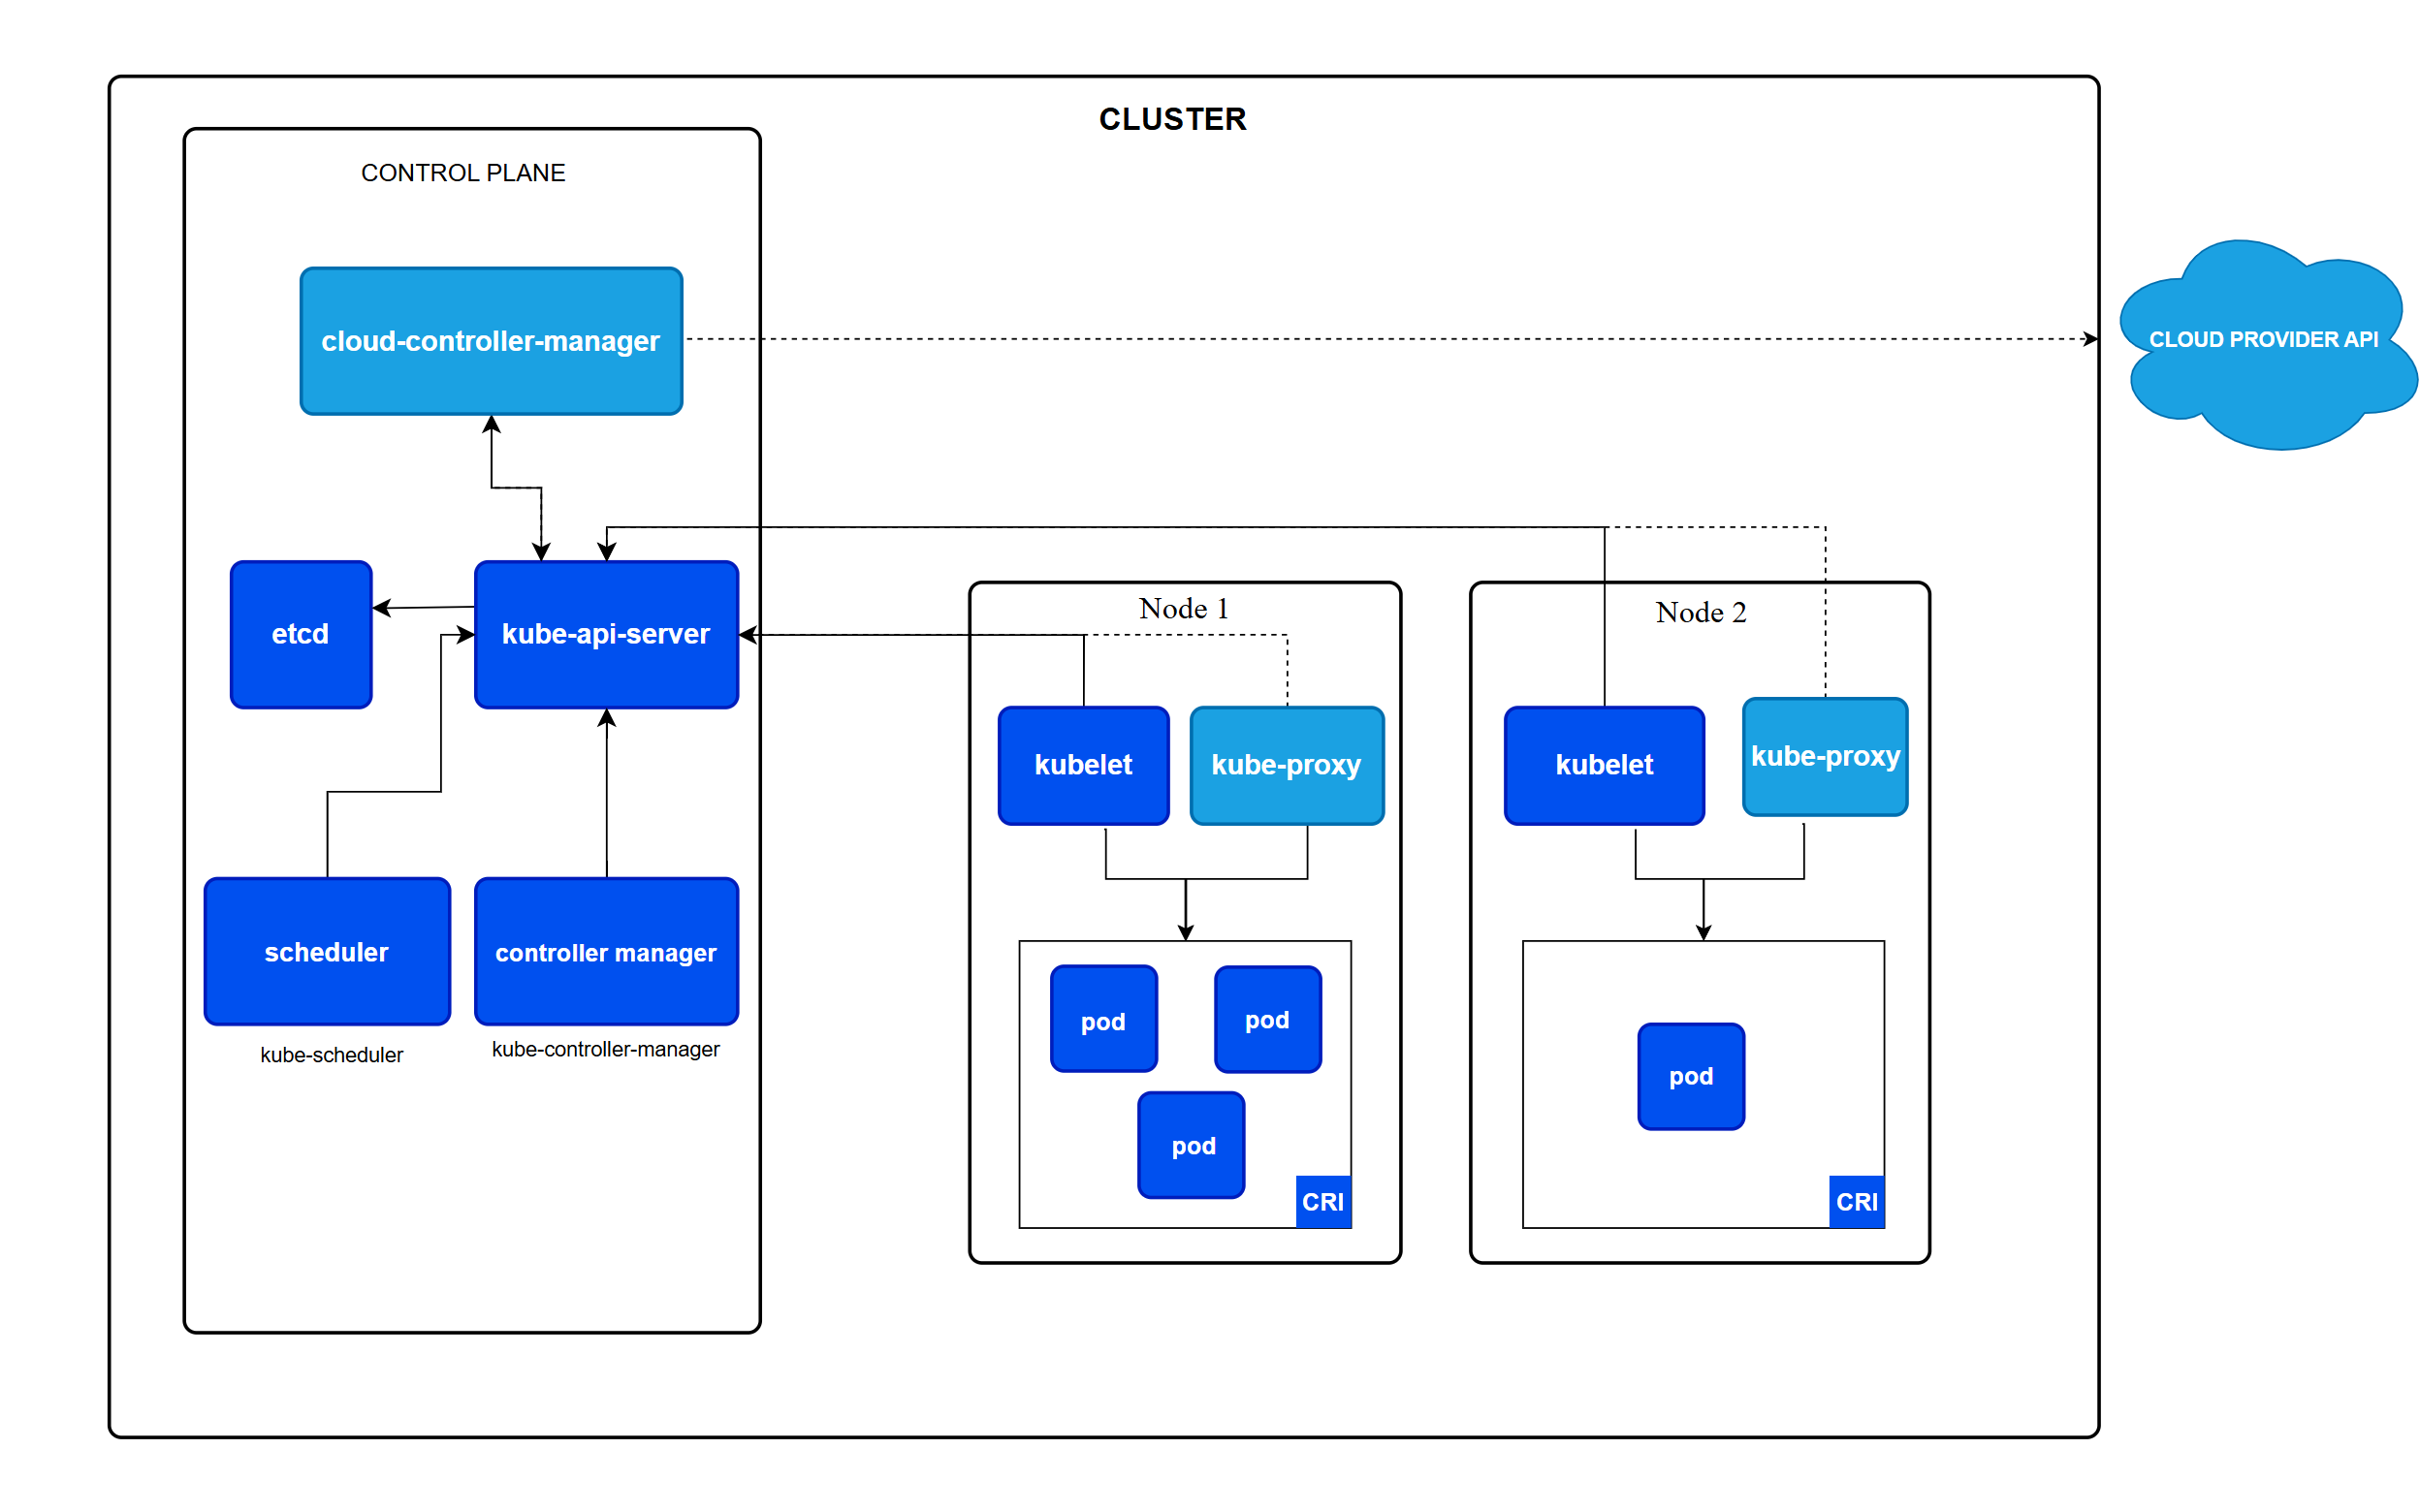
\includegraphics[scale=0.26]{inc/images/kubernetes-cluster-architecture}
    \caption{Компоненты кластера Kubernetes \cite{KubernetesArchSVG}.}
    \label{fig:kubernetes_arch}
\end{figure}

В архитектуре кластера принято выделять два основных типа узлов:

\begin{itemize}
    \item \textbf{Узлы плоскости управления (Control Plane nodes)} — узлы, на которых размещаются компоненты, отвечающие за управление состоянием кластера, планирование рабочих нагрузок и контроль выполнения задач.
    \item \textbf{Рабочие узлы (Worker nodes)} — узлы, на которых непосредственно запускаются контейнеры приложений и выполняются рабочие нагрузки.
\end{itemize}

\subsubsection{Компоненты плоскости управления}

Плоскость управления Kubernetes (Control Plane) обеспечивает централизованное управление кластером и поддерживает согласованность его состояния. Основные компоненты плоскости управления включают следующие элементы.

\textbf{API-сервер (kube-apiserver)} является центральным компонентом архитектуры Kubernetes и выступает в качестве интерфейса взаимодействия между пользователями, внутренними компонентами системы и кластером. Все операции управления кластером выполняются через API-сервер с использованием REST API \cite{KubernetesAPIServer}. kube-apiserver принимает входящие запросы, выполняет их аутентификацию и авторизацию, проверяет корректность данных и записывает изменения состояния кластера в распределённое хранилище. Кроме того, API-сервер является источником audit-логов, фиксирующих информацию обо всех обращениях к API кластера.

\textbf{etcd} представляет собой распределённое отказоустойчивое хранилище типа «ключ–значение», предназначенное для хранения конфигурации и текущего состояния кластера. В etcd сохраняются сведения о ресурсах Kubernetes, таких как поды, сервисы, пространства имён и другие объекты. Все изменения состояния системы сначала фиксируются в etcd, после чего становятся доступными другим компонентам плоскости управления.

\textbf{kube-scheduler} — компонент, отвечающий за планирование рабочих нагрузок. Его задача заключается в выборе наиболее подходящего рабочего узла для размещения нового пода. Планировщик анализирует требования пода к ресурсам, текущую загрузку узлов, политики размещения и ограничения, после чего принимает решение о назначении пода на конкретный узел.

\textbf{kube-controller-manager} представляет собой набор контроллеров, которые отслеживают состояние объектов кластера и обеспечивают его соответствие заданному конфигурационному состоянию. Контроллеры реализуют механизм обратной связи, автоматически исправляя отклонения между текущим и желаемым состоянием системы.

Среди наиболее важных контроллеров можно выделить:

\begin{itemize}
    \item \textbf{Node Controller} — контроллер, отслеживающий состояние рабочих узлов и реагирующий на их отказ или недоступность;
    \item \textbf{Replication Controller} и \textbf{Deployment Controller} — контроллеры, обеспечивающие поддержание заданного числа экземпляров подов;
    \item \textbf{Job Controller} — контроллер, управляющий выполнением пакетных заданий;
    \item \textbf{Service Account Controller} — контроллер, отвечающий за создание сервисных аккаунтов и токенов доступа.
\end{itemize}

\textbf{Cloud Controller Manager} используется в облачных средах и обеспечивает интеграцию Kubernetes с инфраструктурой облачного провайдера, включая управление сетевыми ресурсами, балансировщиками нагрузки и хранилищами.

\subsubsection{Компоненты рабочих узлов}

Рабочие узлы (Worker nodes) предназначены для непосредственного выполнения контейнеризированных приложений. Каждый рабочий узел включает несколько ключевых компонентов.

\textbf{kubelet} — основной агент узла, который обеспечивает взаимодействие рабочего узла с плоскостью управления. kubelet получает инструкции от API-сервера и отвечает за запуск, остановку и мониторинг контейнеров на узле.

\textbf{kube-proxy} — компонент, реализующий функциональность сервисов в Kubernetes. Он отвечает за маршрутизацию сетевого трафика между подами и сервисами, обеспечивая балансировку нагрузки и корректную доставку запросов.

\textbf{Container Runtime} — среда выполнения контейнеров, используемая для запуска и управления контейнерами на узле. В современных кластерах Kubernetes наиболее распространёнными реализациями являются containerd и CRI-O.

\subsubsection{Взаимодействие компонентов кластера}

Взаимодействие между компонентами Kubernetes осуществляется через API-сервер, который выступает центральной точкой управления системой. Пользователи, автоматизированные сервисы и внутренние компоненты отправляют запросы к API-серверу, который проверяет их корректность и вносит изменения в состояние кластера, записывая их в хранилище etcd.

Рабочие узлы регулярно взаимодействуют с API-сервером для получения информации о назначенных им задачах и передачи данных о состоянии запущенных подов. Контроллеры плоскости управления, в свою очередь, анализируют состояние объектов и выполняют действия, направленные на поддержание заданной конфигурации системы.
